\documentclass[11pt]{article}
\usepackage[margin=1in]{geometry}

% Core packages
\usepackage{amsmath,amssymb}
\usepackage{booktabs}
\usepackage{graphicx}
\usepackage{tabularx}
\usepackage{xcolor}
\usepackage[numbers,sort&compress]{natbib}
\usepackage[hidelinks]{hyperref}
\usepackage{subcaption}
\usepackage{float}
\usepackage{placeins}
\usepackage[strings]{underscore}
\graphicspath{{figures/}}

% Paragraphs
\setlength{\parindent}{0pt}
\setlength{\parskip}{0.65\baselineskip}

\newcommand{\bigO}{\mathcal{O}}

\title{Bigger Bird: Context-Aware Sparse Attention for Efficient Long-Context Scaling}
\author{University of Toronto Machine Intelligence Student Team (UTMIST)}
\date{January 2026 -- Present}

\begin{document}
\maketitle

\begin{abstract}
The quadratic cost of dense self-attention limits efficient scaling of
Transformer models to long contexts. We present Bigger Bird, a context-aware
sparse attention mechanism that combines attention sinks, a sliding local
window, and content-based routing of distant key--value positions, where
routing scores are derived from mean causal attention probabilities over a
late-prompt query set. Our Triton kernel implements 64 sink tokens, a
16{,}384-token local window, a per-head routed budget of up to 512 positions,
and exact dense attention over the final 256 prompt queries. We evaluate the
method under a paired dense baseline on BF16 R1-Distill-Llama-8B across
1{,}178 long-context examples from LongCodeQA, Code.Debug, and LongBench~v2.
Pooled accuracy is 34.6\% for Bigger Bird versus 35.3\% for dense attention,
while mean prefill throughput improves by $1.09$--$1.27\times$ on the longer
subsets. A complementary no-KV-cache LongCodeQA pilot at 542K--878K tokens
yields a $10.23\times$ mean prefill speedup on 18 prompts. Prior prototype screens and encoder-scale IMDb / kernel experiments are
retained as developmental evidence: they document the architecture search,
early scaling behavior, and design rationale behind the current method. The
present draft emphasizes inference-time evaluation; sparse-attention training
is left to future work.
\end{abstract}

\newpage
\tableofcontents

\newpage
\section{Introduction}

Transformer models rely on self-attention to connect each token with every
other token in a sequence. Dense self-attention forms an $n\times n$ attention
matrix, giving it $\bigO(n^2)$ comparison and memory cost in sequence length
$n$ \citep{vaswani2017attention}. This quadratic dependence is a practical
bottleneck for long-context inference and for any future training regime that
must process long documents end to end.

Bigger Bird investigates context-aware sparse attention as an alternative to
paying this cost uniformly. Rather than committing to a fixed sparse graph, the
method allocates computation to early attention sinks, a recent local window,
and a content-selected set of distant key--value positions. The current system
of record is \textbf{Bigger Bird v3}: a training-free Triton sparse-prefill
kernel for decoder LLMs, evaluated under a paired dense baseline on
R1-Distill-Llama-8B. Decode remains exact on the retained KV cache; optional
KV eviction and related memory savers are studied as complementary
inference-time mechanisms.

The project developed through a broader architecture search. Experiments~0--15
cover encoder-scale prototypes on BART / BigBird-RoBERTa
\citep{zaheer2020bigbird}; Experiments~16--19 extend the sparse-attention
search on R1; Experiment~20 is the real long-context benchmark suite; and
Experiment~21 studies routing reuse and cache variants. After situating the work in the literature (Section~\ref{sec:related}),
this draft presents the Bigger Bird v3 method, the experimental setup, the
primary R1 results, and the developmental encoder evidence that explains how
the project arrived at the current design.

\section{Related Work}
\label{sec:related}

\paragraph{Fixed sparse patterns.}
Early efficient-attention methods restrict each query to a predefined set of
keys. Sparse Transformers \citep{child2019sparse} factorize attention into
strided and fixed patterns, lowering its cost to $\bigO(n\sqrt{n})$.
Longformer \citep{beltagy2020longformer} and BigBird \citep{zaheer2020bigbird}
combine a sliding window with a small number of global tokens, and BigBird
adds random connections. Both were pretrained with these patterns and can
replace full self-attention in encoder models for document-level tasks. A
separate line of work approximates the full attention matrix rather than
sparsifying it: Linformer \citep{wang2020linformer} projects keys and values
to a fixed length, and Performer \citep{choromanski2021performer} estimates
softmax attention with random features. Among our experiments, the windowed
designs in Experiments~2, 3, and~9 are closest to the sparse-pattern family;
Experiment~2 also adds a linear-attention global path
\citep{qin2024lightning}, and Experiment~15 starts directly from a BigBird
checkpoint.

\paragraph{Content-based routing.}
A second line of work lets the input decide which positions interact.
Reformer \citep{kitaev2020reformer} groups similar queries and keys with
locality-sensitive hashing, and the Routing Transformer
\citep{roy2021routing} assigns them to clusters with online $k$-means and
restricts attention to each cluster. Experiments~1, 4, 6, 10, and~14 share
this principle but score keys directly, either through a low-rank projection
or through pooled block summaries, and keep the top-$k$. More recent work
applies block-level routing at the scale of large language models: Native
Sparse Attention \citep{yuan2025nsa}, which Experiment~11 reimplements,
combines compressed, selected, and sliding-window branches, while MoBA
\citep{lu2025moba} routes each query to a few key blocks with a gate modeled
on mixture-of-experts layers.

\paragraph{Token pruning.}
Instead of thinning the attention pattern, token-pruning methods shorten the
sequence itself. PoWER-BERT \citep{goyal2020powerbert} and learned token
pruning \citep{kim2021tokenpruning} remove tokens judged uninformative as
depth increases, so later layers operate on fewer positions. Token Dropping
(Experiment~8) and Dynamic Context (Experiment~13) take the same approach,
using the $\ell_2$ norm of each hidden state as the importance score.

\paragraph{Attention sinks.}
\citet{xiao2024streamingllm} observed that pretrained language models direct
a large share of attention to the first few tokens even when those tokens
carry little meaning, and that keeping these ``attention sinks'' alongside a
recent window stabilizes long-stream generation without fine-tuning.
Experiment~12 likewise keeps a fixed set of sink tokens visible to every
query, and Experiment~9 always attends to anchor tokens at the start, middle,
and end of the sequence.

\paragraph{Diversity-aware selection.}
The selection rules in the earlier Bigger Bird encoder designs come from
information retrieval and summarization. Maximal marginal relevance
\citep{carbonell1998mmr} trades relevance against redundancy when ranking
candidates, and facility location is a standard submodular objective for
choosing a representative subset \citep{lin2011submodular}. Experiment~5 uses
MMR to choose local keys, while Experiment~15 and the BigBird-family ablation
also use facility location to choose global keys.

\paragraph{Inference-time sparse attention and cache compression.}
Recent decoder-side methods sparsify or compress attention without full
retraining. MInference assigns heads to sparse pattern families at inference
time; SnapKV evicts KV entries using attention near the prompt end; and
DeepSeek's DSA uses a lightweight indexer to select top-$k$ KV entries per
query. Hierarchical summary routers such as LSA and ZHA are related future
comparisons. Bigger Bird v3 is closest to content-based selection with sinks
and a local window, but routes from late-prompt query attention rather than a
separately trained indexer.

\section{Method}
\label{sec:methodology}
\label{sec:method}

This section states the current Bigger Bird v3 design first, then summarizes
the architecture search that produced it. Evaluation suites, protocols, and
metrics are in Section~\ref{sec:setup}.

\subsection{Bigger Bird v3}
\label{exp:bb-v3}
\label{sec:method-v3}

Bigger Bird v3 is the current method of record: a training-free sparse-prefill
attention for decoder LLMs. The design goal is to preserve useful long-range
links while avoiding a full causal attention matrix over the prompt.

Default configuration:
\texttt{\{"sink":64, "window":16384, "vertical":512, "exact\_tail":256\}}.
For each layer, every query attends to
\begin{itemize}
  \item the first 64 tokens (attention sinks);
  \item the previous 16{,}384 tokens (local window);
  \item up to 512 distant positions per head, selected from mean causal
    attention probability over the final 64 prompt queries (content-based
    routing);
  \item and, for the final 256 prompt queries, exact attention over their
    visible prefix (exact tail).
\end{itemize}
Decode is exact on the retained KV cache. Optional KV eviction and memory
savers (chunked MLP, CPU embeddings, INT8 KV) are complementary inference
mechanisms, not part of the core attention pattern. The implementation lives
in \texttt{modal\_rd/attention.py} with the Triton kernel in
\texttt{kernels/bigger\_bird\_flash.py}.


\subsection{Prior architecture search}
\label{sec:architectures}

Table~\ref{tab:taxonomy} summarizes the broader search that led to Bigger Bird
v3. Experiments~0--15 are encoder-scale prototypes; Experiments~16--21 are the
later R1 / long-context line. Brief mechanism notes follow; measured outcomes
appear in Sections~\ref{sec:results} and~\ref{sec:developmental}.

\begin{table}[ht]
  \centering
  \caption{Taxonomy of evaluated attention mechanisms (Experiments~0--21 and
  Bigger Bird v3).}
  \label{tab:taxonomy}
  \begin{tabularx}{\textwidth}{@{}l>{\raggedright\arraybackslash}Xl@{}}
    \toprule
    Family & Representative mechanism & Experiments \\
    \midrule
    Reference & Dense self-attention (BART; later HF SDPA on R1) & 0 \\
    Routed sparse & Low-rank top-$k$, block routing, GQA routing,
      coarse-to-fine & 1, 4, 6, 10, 17 \\
    Adaptive computation & Layer schedules, token dropping, dynamic context
      & 7, 8, 13, 14 \\
    Hybrid / multi-branch & Windows, globals, speculation, NSA, S2-HHST,
      free NSA, confidence-gated & 2, 3, 9, 11, 12, 16, 18 \\
    Encoder Bigger Bird & MMR / facility-location / teleports on BART or
      BigBird-RoBERTa & 5, 15 \\
    Decoder Bigger Bird & Flash / Triton sparse prefill; sinks + window +
      routed distant keys + exact tail & 19, v3 \\
    Long-context systems & Real-benchmark harness; routing reuse / KV
      eviction variants & 20, 21 \\
    \bottomrule
  \end{tabularx}
\end{table}

Experiments~11 and~12 began as unfinished prototypes. Experiment~20 is the
real-benchmark harness used in Section~\ref{sec:results}; Experiment~21 studies
routing reuse and KV-cache variants.


\subsubsection*{Experiment 0: Dense Baseline}
\label{exp:baseline}
Standard dense self-attention, every query attending to every key:
$\mathrm{Attention}(Q,K,V) = \mathrm{softmax}(QK^\top/\sqrt{d})V$. Early
encoder runs used BART \citep{lewis2020bart}; the current R1 baseline is
Hugging Face SDPA on R1-Distill-Llama-8B. This remains the reference for
quality and resource comparisons. \emph{Complexity:} $\bigO(n^2)$ compute and
memory in sequence length $n$.

\subsubsection*{Experiment 1: DeepSeek Top-k Routing}
\label{exp:deepseek}
A custom head-shared, low-rank router first scores all keys cheaply in a
reduced dimension, then selects a fixed number of top-scoring keys per head;
each query attends only to that shared key set under full-dimensional
attention. The defaults are $d_{\mathrm{low}}=16$ and top-$k=64$, with the
same keys reused across query positions in each head. The method falls back to
dense attention on short sequences. Although named after DeepSeek, it is an
adaptation rather than a direct implementation of Multi-head Latent Attention
\citep{deepseek2024v3}. \emph{Complexity:}
$\bigO(n\,d_{\mathrm{low}}+nKd)\approx\bigO(n)$ for fixed $K$.

\subsubsection*{Experiment 2: Lightning Hybrid}
\label{exp:lightning}
Combines an unfolded sliding-window local softmax, without materializing the
full $T\times T$ score matrix, with an optional linear-attention global path
using the feature map $\mathrm{elu}(x)+1$ \citep{qin2024lightning}. The global
path activates when the sequence exceeds four times the default 128-token
window, and its output is added to the local contribution.
\emph{Complexity:} $\bigO(nW)$ locally and $\bigO(nW+nd^2)$ with the global
path.

\subsubsection*{Experiment 3: Dynamic Global Tokens}
\label{exp:dynglobal}
A learned linear gate scores every token's ``globalness''; the top-scoring
tokens are selected once per batch as global tokens, and every query attends
to this learned global set plus a local sliding window in a single softmax.
\emph{Defaults:} $G=16$ global tokens, window size $W=64$.
\emph{Complexity:} $\bigO(n\,(G+W)\,d) = \bigO(n)$ for fixed $G,W$.

\subsubsection*{Experiment 4: PBS Attention}
\label{exp:pbs}
Queries and keys are mean-pooled into blocks, a head-shared block router
selects the top-scoring blocks, and tokens from those blocks are gathered with
sorted indices for coalesced GPU access before sparse softmax. The default is
two 64-token blocks, or 128 selected keys. \emph{Complexity:}
$\bigO(n_{\mathrm{blocks}}B+nMBd)\approx\bigO(n)$ for fixed block size $B$
and selected-block count $M$.

\subsubsection*{Experiment 5: Unified Bigger Bird (BART backbone)}
\label{exp:unified-bb}
Patches BART self-attention with one combined selection pattern: MMR-lite
diversity-aware local top-$k$ selection \citep{carbonell1998mmr}, a learned
gate that chooses global tokens, and biased random teleports that mix
high-gate candidates with uniformly sampled positions. Each query attends
only to the union of local selections, globals, and teleports. The learned
global gate deliberately differs from Experiment~15, which uses a submodular
facility-location objective.

\subsubsection*{Experiment 6: DeepSeek + PBS Hybrid}
\label{exp:deepseekpbs}
Combines content-aware routing with GPU-friendly block coalescing: low-rank
query/key projections (as in Experiment~1) first identify the top-scoring
blocks (as in Experiment~4), and top-$k$ tokens are then selected \emph{within}
those blocks; selected indices are sorted to guarantee contiguous memory
reads.

\subsubsection*{Experiment 7: Layer-Adaptive Sparsity}
\label{exp:layer-adaptive}
Uses a per-layer key budget that begins with broad attention and becomes more
sparse in later layers, reflecting the hypothesis that early layers require
more context for feature extraction while later layers can reason over fewer
selected tokens. The default budgets are 192 keys in early layers, 64 in
middle layers, and 32 in late layers.

\subsubsection*{Experiment 8: Token Dropping}
\label{exp:token-drop}
Runs three ordinary dense attention layers to extract local features, scores
each token's importance by the $\ell_2$ norm of its hidden state, and drops
the bottom 30\% of tokens before continuing with a shorter sequence for the
remaining layers. \emph{Complexity:} attention cost after the drop point
scales with $\mathrm{keep\_ratio}^2$ relative to the undropped sequence. This
follows the broader token-pruning literature \citep{goyal2020powerbert,kim2021tokenpruning}.

\subsubsection*{Experiment 9: Attention Speculation}
\label{exp:speculation}
Inspired by speculative decoding \citep{leviathan2023speculative}. Every layer runs a sparse ``fast path''
(local window plus first/middle/last anchor tokens); every fourth layer
additionally computes full dense attention as a verifier and adds a
KL-divergence distillation loss that trains the fast path to mimic full
attention. At inference, only the fast path executes.

\subsubsection*{Experiment 10: Grouped-Query Sparse Attention}
\label{exp:gqa}
Stacks two memory-saving mechanisms: (a) grouped-query attention compresses
12 key/value heads into 4 shared groups via mean pooling (a 3$\times$ memory
reduction), and (b) top-$k$ sparse routing is applied on top of the shared
groups, so softmax cost drops from $\bigO(N)$ to $\bigO(K)$ per query
\citep{ainslie2023gqa}.

\subsubsection*{Experiment 11: Native Sparse Attention (NSA)}
\label{exp:nsa}
Combines three parallel branches -- compressed (pooled) attention, explicitly
selected-block attention, and sliding-window attention -- whose outputs are
combined per query. This experiment is marked incomplete (``TODO'') in the
codebase at the time of this report; see the note at the start of
Section~\ref{sec:architectures} and the original NSA design
\citep{yuan2025nsa}.

\subsubsection*{Experiment 12: S2-HHST}
\label{exp:s2hhst}
Shard-based hierarchical sparse attention with dedicated sink tokens: the
sequence is partitioned into shards, attention is computed hierarchically
within and across shards, and fixed sink tokens are always visible. This
experiment is likewise marked incomplete (``TODO'') in the codebase; see the
note at the start of Section~\ref{sec:architectures}.

\subsubsection*{Experiment 13: Dynamic Context}
\label{exp:dynamic-context}
Extends Token Dropping to arbitrarily long inputs. After three dense early
layers, tokens are scored by hidden-state $\ell_2$ norm and exactly 4096 are
retained regardless of the original length. Inputs longer than 8192 tokens
are processed independently by chunk in the early layers, avoiding a full
input-length attention matrix; late layers always attend over the fixed
budget. \emph{Complexity:}
$\bigO(\mathrm{num\_chunks}\times\mathrm{chunk\_size}^2)$ for early layers
plus $\bigO(\mathrm{budget}^2)$ for late layers.

\subsubsection*{Experiment 14: Token Drop + DeepSeek Routing}
\label{exp:token-drop-deepseek}
Combines Token Dropping with the DeepSeek-style low-rank router for two levels
of sparsity. Early layers run densely, 30\% of low-importance tokens are
dropped after layer 3, and subsequent layers apply top-$k$ routing to the
shortened sequence. Defaults are top-$k=64$ and low-rank dimension 16.

\subsubsection*{Experiment 15: Proper Bigger Bird (BigBird-RoBERTa backbone)}
\label{exp:proper-bb}
The original UTMIST Bigger Bird design is built directly on
\texttt{bigbird-roberta-base} \citep{zaheer2020bigbird}. It extends the
middle-block attention path with MMR-lite local top-$k$ selection,
facility-location global selection \citep{lin2011submodular}, and biased
block-wise teleports. Defaults are 128-token fragments, $\max_k=64$, six
globals, and four teleports per head. No standalone task-level run is
available for this exact configuration; the related ablation below uses the
same selection ideas on a BART backbone.

\subsubsection*{BigBird-Family Ablation}
\label{exp:bigbird-family}
This separate study compares stock BigBird \citep{zaheer2020bigbird} with a
BART-based hybrid using blocked-MMR local selection, facility-location
globals, and optional teleports. It evaluates globals alone, local MMR alone,
a refined MMR rule, and combinations of MMR, globals, random links, and
teleports. Because its backbone differs from Experiment~15 and its global
selector differs from Experiment~5, the results isolate selection mechanisms
rather than directly compare the numbered Bigger Bird implementations.

\subsubsection*{Experiment 16: Free NSA}
Parameter-free / untrained NSA-style multi-branch routing (window +
compressed + selected). Used as a zero-shot R1 screen; learned compressors
and gates that are never trained fail retrieval in this setting.

\subsubsection*{Experiment 17: Coarse-to-Fine Routing}
Two-stage content routing: select top blocks, then top-$k$ tokens within
those blocks. Screens show that fine-token budget dominates block coverage at
long context.

\subsubsection*{Experiment 18: Confidence-Gated Multi-Resolution}
Local window plus a low-rank causal linear branch and a head-shared routed
global correction. Validation remains preliminary relative to Bigger Bird v3.

\subsubsection*{Experiment 19: Bigger Bird Flash}
An earlier Flash / Triton sparse-prefill prototype that preceded the final
v3 configuration. Retained in screening tables; superseded by Bigger Bird v3
for the main R1 claims.


\subsubsection*{Experiment 20: Real Long-Context Benchmark Harness}
Paired dense / Bigger Bird evaluation on LongCodeQA, Code.Debug, and
LongBench~v2. The full H100 matched suite (1{,}178 examples, 130K prompt cap)
is the primary real-benchmark evidence in Section~\ref{sec:r1-benchmark}.

\subsubsection*{Experiment 21: Kascade / Cache Variants}
Follow-up study of routing reuse across layers and KV-cache eviction /
compression at long context, including held-out fact retention probes near
1M tokens. Cross-layer route reuse is incompatible with per-layer eviction
when cache slots no longer refer to the same tokens.


\section{Experimental Setup}
\label{sec:setup}
\label{sec:dataset}

The evaluation has four aims: (i)~test whether context-aware sparse prefill
preserves dense answer quality on real long-context benchmarks;
(ii)~measure prefill time, decode speed, and peak memory under a matched dense
baseline into the 32K--130K regime, with pilots beyond 500K tokens;
(iii)~identify which routing mechanisms survive synthetic retrieval screens;
and (iv)~retain encoder-scale IMDb / LRA runs as developmental rationale and
small-scale scaling evidence
(Section~\ref{sec:developmental}).

\subsection{Evaluation suites}

\textbf{Primary (current).} The main quantitative claims use BF16
R1-Distill-Llama-8B under a paired dense baseline:
\begin{itemize}
  \item \textbf{LongCodeQA} repository comprehension (32K / 64K / 128K
    buckets, plus a 1M-token pilot);
  \item \textbf{InfiniteBench Code.Debug} bug localization;
  \item \textbf{LongBench~v2} multi-domain long-context reasoning;
  \item synthetic \textbf{RULER} needle-in-a-haystack screens used during
    method development \citep{hsieh2024ruler}.
\end{itemize}
Accuracy on the real suites is the first-token A--D choice. Prefill is a
full-prompt forward; decode timing uses a short CUDA-graph probe and is not a
patch-success metric.

\textbf{Developmental (supporting).} Earlier work used \textbf{IMDb}
sentiment classification on BART / BigBird-RoBERTa at fixed lengths
\citep{maas2011imdb}, plus exploratory \textbf{Long Range Arena (LRA)}
ListOps and Text runs \citep{tay2021lra}. Those smaller-scale experiments
document how the project searched architectures, observed early scaling
trends, and chose content-aware routing. They explain how we arrived at
Bigger Bird v3; they are not the primary long-context claim.

\subsection{Experimental Protocol}
\label{sec:protocol}

\paragraph{Current R1 protocol.}
Primary runs use BF16 R1-Distill-Llama-8B on H100 80~GB under a paired dense
baseline (HF SDPA) versus Bigger Bird v3. Prompts are capped at 130{,}000
tokens (middle-truncated where necessary). Prefill is a full-prompt forward
with MLP chunking (8{,}192); decode timing uses a 16-step greedy CUDA-graph
probe. Accuracy is the first answer-token distribution renormalized over
A--D. The matched suite completed every listed item in both arms with no OOM
(final report dated 2~Nov~2026). A separate LongCodeQA 1M pilot uses
no-KV-cache full-prompt forwards on identical untruncated prompts.

\paragraph{Developmental encoder protocol.}
Earlier work used an isolated attention-kernel benchmark (CUDA, 10 timing
trials, 128--32{,}768 tokens) and BART fine-tuning on IMDb at fixed lengths
(256--65{,}536 tokens), recording F1, accuracy, training time, peak memory,
and inference latency. Length and metric coverage vary by architecture;
comparisons are made only at matched lengths. Those runs remain single-seed
estimates and are treated as developmental evidence.

\subsection{Metrics}
\label{sec:metrics}

Table~\ref{tab:metrics} defines the metrics used in this draft. For the
current R1 claims, A--D accuracy, prefill time, decode ms/token, and peak
allocated memory are primary. F1 and related IMDb / kernel metrics apply to
the developmental encoder experiments in Section~\ref{sec:developmental}.

\begin{table}[ht]
  \centering
  \small
  \caption{Metrics used in this report.}
  \label{tab:metrics}
  \begin{tabularx}{\textwidth}{@{}lXll@{}}
    \toprule
    Metric & Interpretation & Unit \\
    \midrule
    A--D accuracy & First-token multiple-choice correctness (R1 suites) & 0--1 \\
    Prefill time & Full-prompt forward latency & s \\
    Prefill ratio & Mean dense prefill / mean Bigger Bird prefill
      ($>1$ favors BB) & $\times$ \\
    Decode speed & CUDA-graph probe latency & ms/token \\
    Peak memory & Max CUDA allocated over prefill (+ short decode) & GB \\
    F1 & IMDb sentiment quality (developmental) & 0--1 \\
    Attention forward time & Isolated kernel runtime (developmental) & ms \\
    Training time & Wall-clock training time (developmental) & s \\
    OOM boundary & Longest completed context without OOM & tokens \\
    \bottomrule
  \end{tabularx}
\end{table}


\section{Results}
\label{sec:results}
\label{sec:r1-benchmark}

This section reports the primary evidence for Bigger Bird v3: matched
long-context evaluation on R1-Distill-Llama-8B, then the synthetic screens and
ablations that connect earlier prototypes to the final design. Developmental
encoder-scale IMDb / kernel experiments follow in
Section~\ref{sec:developmental} as the rationale and scaling scaffold behind
that path.

\subsection{Matched R1 long-context benchmarks}

The tables below summarize the matched H100 evaluation of Bigger Bird v3
against dense attention (BF16 R1-Distill-Llama-8B; final report updated
2~Nov~2026). BB denotes Bigger Bird v3.


We evaluated 1{,}178 paired examples on one H100 80~GB. LongCodeQA tests
repository comprehension, Code.Debug tests bug localization, and LongBench~v2
tests long-context reasoning. Accuracy is the first-token choice among A--D.
Prefill is a full-prompt forward; decode is a separate 16-step CUDA-graph
timing probe.

\begin{table}[ht]
  \centering
  \small
  \caption{Matched R1 benchmark: dense vs.\ Bigger Bird v3 (H100 80~GB, BF16,
  130K prompt cap). Prefill ratio is mean dense time / mean BB time; above
  $1\times$ favors Bigger Bird.}
  \label{tab:r1-benchmark}
  \begin{tabular}{@{}lrrrr@{}}
    \toprule
    Benchmark & $n$ & Accuracy dense / BB & Prefill dense / BB (s) & Prefill ratio \\
    \midrule
    LongCodeQA 32K  & 113 & 67.3\% / 67.3\% & 0.79 / 1.17 & $0.67\times$ \\
    LongCodeQA 64K  & 76  & 63.2\% / 63.2\% & 2.55 / 3.17 & $0.80\times$ \\
    LongCodeQA 128K & 92  & 52.2\% / 51.1\% & 6.07 / 5.59 & $1.09\times$ \\
    Code.Debug      & 394 & 27.7\% / 26.6\% & 8.75 / 6.89 & $1.27\times$ \\
    LongBench v2    & 503 & 26.8\% / 26.0\% & 6.70 / 5.31 & $1.26\times$ \\
    \bottomrule
  \end{tabular}
\end{table}

The 128K bucket has a $0.99\times$ median paired ratio and averages about 88K
actual tokens. Mean decode, dense / Bigger Bird, was 10.42 / 10.41,
12.08 / 12.08, 14.06 / 14.08, 15.33 / 15.34, and 13.76 / 13.77~ms/token,
respectively. Pooled accuracy was 35.3\% / 34.6\% (416/1178 vs.\ 407/1178);
paired McNemar $p \geq 0.683$ does not establish equivalence. Code.Debug and
LongBench~v2 prompts beyond 130K were middle-truncated (136/394 and 186/503).
These scores do not measure patch success.

\begin{table}[ht]
  \centering
  \small
  \caption{KV eviction arm (\texttt{bb\_evict64k}: sink 64 + window 16{,}384 +
  up to 65{,}536 extra selected middle positions). Eviction is applied after
  prefill logits, so first-token QA matches BB v3 by construction.}
  \label{tab:r1-evict}
  \begin{tabular}{@{}lrrr@{}}
    \toprule
    Benchmark & BB / +evict accuracy & Decode BB / +evict (ms/tok) & Peak BB / +evict (GB, mean) \\
    \midrule
    LongCodeQA 32K  & 67.3\% / 67.3\% & 10.41 / 10.53 & 20.9 / 22.9 \\
    LongCodeQA 64K  & 63.2\% / 63.2\% & 12.08 / 12.20 & 25.7 / 30.8 \\
    LongCodeQA 128K & 51.1\% / 51.1\% & 14.08 / 13.71 & 32.3 / 38.4 \\
    Code.Debug      & 26.6\% / 26.6\% & 15.34 / 14.11 & 35.7 / 39.3 \\
    LongBench v2    & 26.0\% / 26.0\% & 13.77 / 12.74 & 31.9 / 34.1 \\
    \bottomrule
  \end{tabular}
\end{table}

\subsection{One-million-token evaluations}

\begin{table}[ht]
  \centering
  \small
  \caption{One-million-token paired evaluations. LongCodeQA: same H100, BF16,
  identical untruncated prompts; paired $p=0.625$. RULER: dense on B200
  (CPU-offloaded KV) vs.\ BB on H100, so no fair prefill ratio.}
  \label{tab:1m-evals}
  \begin{tabular}{@{}lrrrrr@{}}
    \toprule
    Evaluation & $n$ & Tokens & Dense & BB & Prefill (dense $\rightarrow$ BB) \\
    \midrule
    LongCodeQA 1M & 18/50 & 542K--878K & 7/18 (38.9\%) & 9/18 (50.0\%)
      & 470.38 $\rightarrow$ 45.97~s (\textbf{10.23$\times$}) \\
    Synthetic RULER & 18 & 971K--980K & 10/18 (55.6\%) & 9/18 (50.0\%)
      & --- \\
    \bottomrule
  \end{tabular}
\end{table}

\begin{table}[ht]
  \centering
  \small
  \caption{Exp~21 held-out fact retention near 1M tokens (25 prompts,
  4 facts each). No dense BF16 full-cache quality baseline; decode values
  are estimates.}
  \label{tab:1m-exp21}
  \begin{tabular}{@{}lrr@{}}
    \toprule
    Cache setting & Fact recall & Median prefill \\
    \midrule
    Eviction keep 16K  & 62\% & 63~s \\
    Eviction keep 64K  & 85\% & 63~s \\
    Eviction keep 128K & 86\% & 63~s \\
    4-bit full cache   & 91\% & 72--78~s \\
    \bottomrule
  \end{tabular}
\end{table}

The LongCodeQA test is a no-KV-cache full-prompt forward (first-answer logits),
not decoding or cache retention; 32 prompts remain unmeasured. Median paired
prefill ratio on the measured LongCodeQA subset is $9.48\times$.

\subsection{Earlier project screening experiments}

Table~\ref{tab:screening} records an early prototype screen: byte budget
65{,}536, 30 examples, depth 0.5, R1 on an H100 3g.40GB MIG, no KV cache.
The scorer extracts the first number and checks its last digit. Bigger Bird
v3 is \emph{not} in this batch; it was developed afterward under a separate
Modal NIAH protocol (Tables~\ref{tab:v3-niah}--\ref{tab:v3-ablate}).

\begin{table}[ht]
  \centering
  \small
  \caption{Pre-v3 prototype screening on synthetic needle retrieval
  (30 examples). Relative $=$ last-digit accuracy / dense 30/30. Rows marked
  ``each'' apply the listed score to every named experiment. Development
  record, not a fair ranking of published methods.}
  \label{tab:screening}
  \begin{tabular}{@{}>{\raggedright\arraybackslash}p{0.28\linewidth}
                >{\raggedright\arraybackslash}p{0.42\linewidth}rr@{}}
    \toprule
    Screening result & Experiments & Score & Rel. \\
    \midrule
    Dense reference
      & Exp~0
      & 30/30 & 100\% \\
    Content selection / routing
      & Exp~1 Top-k; 10 GQA; 13 DynamicContext; 15 earlier Bigger Bird (\textbf{each})
      & 27/30 & 90\% \\
    Coarse-to-fine
      & Exp~17
      & 22/30 & 73\% \\
    Bigger Bird Flash
      & Exp~19
      & 16/30 & 53\% \\
    Zero-score prototypes
      & Exp~2, 3, 4, 7, 8, 11, 12, 18 (\textbf{each})
      & 0/30 & 0\% \\
    Not selected here
      & Exp~5, 6, 9, 14, 16
      & --- & --- \\
    \bottomrule
  \end{tabular}
\end{table}

\begin{table}[ht]
  \centering
  \small
  \caption{Bigger Bird v3 synthetic NIAH confirmation (Modal; exact-match
  scoring; depth 0.5 unless noted). Final config:
  \texttt{sink=64}, \texttt{window=16384}, \texttt{vertical=512},
  \texttt{exact\_tail=256}. Prompts 0--5 at $\sim$127K were used in tuning;
  held-out is prompts 6--29.}
  \label{tab:v3-niah}
  \begin{tabular}{@{}lrrrrr@{}}
    \toprule
    Context & Arm & Exact (30) & Held-out (24) & Prefill (s) & Ratio \\
    \midrule
    $\sim$65K  & Dense & 30/30 & 24/24 & 5.02 & --- \\
    $\sim$65K  & BB v3 & 30/30 & 24/24 & 4.41 & $1.14\times$ \\
    $\sim$128K & Dense & 28/30 & 22/24 & 16.25 & --- \\
    $\sim$128K & BB v3 & 30/30 & 24/24 & 8.61 & $1.89\times$ \\
    $\sim$128K (depth 0.1) & Dense & 28/30 & 23/24 & 16.39 & --- \\
    $\sim$128K (depth 0.1) & BB v3 & 30/30 & 24/24 & 8.56 & $1.91\times$ \\
    \bottomrule
  \end{tabular}
\end{table}

\begin{table}[ht]
  \centering
  \small
  \caption{Why Exp~19 underperformed relative to v3: matched tuning-set
  prompts at $\sim$127K (depth 0.5, $n{=}6$). Exact-tail ablation uses a 4K
  window; final v3 uses the 16K window.}
  \label{tab:v3-ablate}
  \begin{tabular}{@{}lrr@{}}
    \toprule
    Configuration & Exact & Prefill (s) \\
    \midrule
    Dense & 6/6 & 16.33 \\
    Exp~19 Bigger Bird Flash & 0/6 & 4.33 \\
    Exact tail $=0$ (4K window) & 2/6 & 4.95 \\
    Exact tail $=64$ (4K window) & 4/6 & 5.45 \\
    Exact tail $=256$ (4K window) & 6/6 & 6.09 \\
    BB v3 final (16K window) & 6/6 & 8.50 \\
    \bottomrule
  \end{tabular}
\end{table}

Table~\ref{tab:v3-niah} shows that the final v3 config recovers dense-level
needle retrieval while nearly doubling prefill speed at $\sim$128K.
Table~\ref{tab:v3-ablate} links Exp~19's weak screen to missing coverage:
without a sufficient exact tail, the same development prompts fail even when
prefill is fast. These synthetic results motivate the design; the primary
real-benchmark claim remains Section~\ref{sec:r1-benchmark}.


\section{Developmental Encoder Experiments}
\label{sec:developmental}

This section keeps the encoder-scale architecture search (BART /
BigBird-RoBERTa) that preceded the R1 line. These were smaller experiments
than the H100 suite, but they are how the project reached Bigger Bird v3:
they established the team's sparse-attention workflow, made early scaling
trends in kernel time, latency, memory, and training cost visible, and
supplied the rationale for favoring content-based routing over fixed or
untrained selection alone. They support the path to Section~\ref{sec:results};
they do not replace it.

\subsection{Per-architecture outcomes}

The following summary records the strongest and weakest measured outcomes for
each early architecture. Detailed efficiency tables follow in
Section~\ref{sec:efficiency}; complete developmental tables are in the
appendix.

\textbf{Dense Baseline (Experiment 0).} The baseline reaches its best IMDb F1
of 0.931 at 768 tokens and 0.917 at 16{,}384 tokens. Its isolated attention
kernel requires 95.4~ms at 16{,}384 tokens and OOMs at 32{,}768; at task level
it completes 32{,}768 tokens using 20.6~GB and 925~ms per sequence, but fails
at 65{,}536 tokens.

\textbf{DeepSeek Top-k Routing (Experiment 1).} The kernel is
2.3--4.6$\times$ faster than dense attention from 1024 to 4096 tokens and
17.4$\times$ faster at 16{,}384. Task quality is uneven: several runs reach
F1 0.82--0.86, while the 2048-token run falls to 0.519 and the 32{,}768-token
run collapses to F1 0.

\textbf{Lightning Hybrid (Experiment 2).} Its measured kernel remains slower
than dense attention, including 34.4~ms versus 27.1~ms at 4096 tokens, and
several task-level runs collapse to F1 0. It is therefore more useful as an
implementation diagnostic than as a leading candidate.

\textbf{Dynamic Global Tokens (Experiment 3).} Kernel time is below dense
attention at 4096 tokens, but task quality is unstable: a strong 512-token run
is followed by majority-class collapses at multiple longer lengths. The
learned global gate is not yet reliable across configurations.

\textbf{PBS Attention (Experiment 4).} Block routing becomes faster than
dense attention from 1024 tokens onward and approaches DeepSeek Top-k kernel
time at 4096 tokens. However, several IMDb runs collapse to F1 0, so its
kernel efficiency does not translate consistently to task quality.

\textbf{Unified Bigger Bird (Experiment 5).} At 768 tokens it reaches F1
0.926 versus 0.931 for dense attention, but requires 12.8$\times$ more
training time. Several 1024--2048-token runs collapse and the recorded
configuration OOMs at 4096 tokens. Section~\ref{sec:bigbird-family-results}
compares related Bigger Bird variants.

\textbf{DeepSeek + PBS Hybrid (Experiment 6).} Recorded IMDb runs from 512 to
4096 tokens collapse to majority-class prediction despite favorable nominal
comparison counts. The architecture is therefore classified as unsuccessful
in its current implementation.

\textbf{Layer-Adaptive Sparsity (Experiment 7).} This is the most consistent
sparse method: F1 is 0.891 at 1024 tokens versus 0.894 for dense attention and
0.864 at 4096 versus 0.909, while its kernel is 2.3--4.0$\times$ faster through
4096 tokens and 17.5$\times$ faster at 16{,}384.

\textbf{Token Dropping (Experiment 8).} This method has the strongest
long-context resource profile. At 8192 tokens it is 3.28$\times$ faster in
inference and uses 42.3\% less memory than dense attention; at 32{,}768 the
advantages grow to 3.47$\times$ and 82.5\%. It is the only method with a
completed 65{,}536-token IMDb run.

\textbf{Attention Speculation (Experiment 9).} Available quality is
reasonable at 1024--2048 tokens, but memory reaches 9.4~GB at 2048 and the
method OOMs at 4096 tokens.

\textbf{Grouped-Query Sparse Attention (Experiment 10).} The kernel scales
well, reaching 2.2--3.9$\times$ speedups from 1024 to 4096 tokens and about
17$\times$ at 16{,}384. Task-level runs remain unstable, with both useful and
collapsed configurations.

\textbf{Native Sparse Attention (Experiment 11).} One short-context run
achieves strong IMDb quality, but its recorded training time is far above
other methods and most latency and memory fields are missing. Because the
implementation is marked unfinished, these values are preliminary.

\textbf{S2-HHST (Experiment 12).} Available short-context runs reach moderate
IMDb quality with training time somewhat above the dense baseline, but memory
and latency are not recorded. Its unfinished status also limits conclusions.

\textbf{Dynamic Context (Experiment 13).} This method produces the strongest
IMDb quality result, F1 0.942 at 1024 tokens, together with 5.35~ms latency
versus 13.18~ms for dense attention. The trade-off is nearly 10$\times$ longer
training. On RULER it retrieves perfectly at 4096 tokens but degrades sharply
at longer contexts.

\textbf{Token Drop + DeepSeek Routing (Experiment 14).} The method retains
competitive LRA Text F1 through 4096 tokens, but recorded memory is high and
longer configurations OOM. Its evaluation settings also differ from the
Bigger Bird runs, preventing direct chart comparison without re-evaluation.

\textbf{Proper Bigger Bird (Experiment 15).} No standalone IMDb run is
reported for the exact BigBird-RoBERTa configuration. The closest evidence is
the BART-based BigBird-family ablation, which shares its MMR,
facility-location, and teleport mechanisms but should not be treated as a
direct measurement of Experiment~15.

\subsection{Highlighted models and early scaling plots}

The developmental graphs focus on four representative models from the early
search: the Dense Baseline as reference, Unified Bigger Bird as the then-target
architecture, and two strong sparse alternatives by measured overall score
(Dynamic Context and Token Dropping). For kernel-only plots, Layer-Adaptive
Sparsity replaces Dynamic Context because Dynamic Context was not in the
kernel benchmark.

These plots are useful as early scaling evidence: Layer-Adaptive gave the
most consistent IMDb quality--kernel-speed balance, Token Dropping scaled best
to very long encoder contexts, and Dynamic Context produced the highest
short-context IMDb F1. Several other methods had fast kernels but unstable
task quality. Full per-experiment tables, including failed and incomplete
runs, are in Tables~\ref{tab:app-kernel} and~\ref{tab:app-imdb}.

\subsection{Log-Log Attention Forward Time}
\label{sec:loglog}

\begin{figure}[ht]
  \centering
  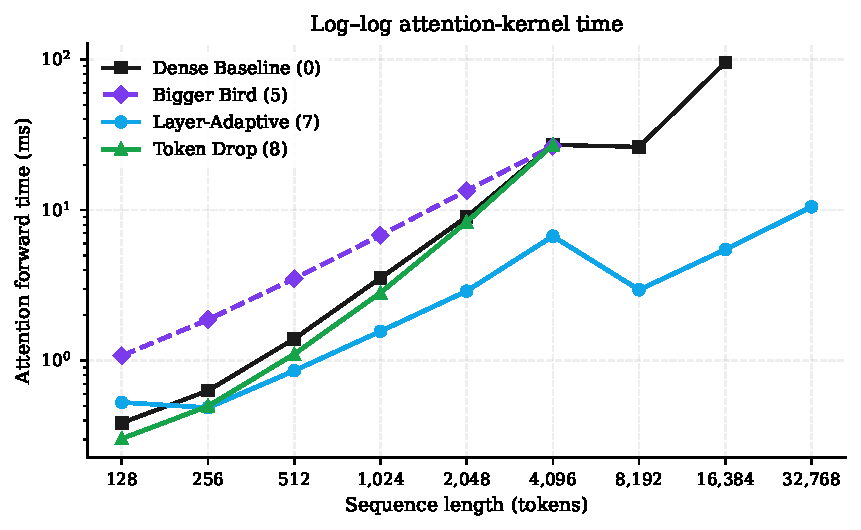
\includegraphics[width=\linewidth]{sel_loglog}
  \caption{Log--log attention-kernel time for four experiments: Dense
  Baseline (0), Bigger Bird Unified (5), Layer-Adaptive Sparsity (7), and
  Token Dropping (8). Layer-Adaptive, Token Dropping, and the dense baseline
  extend to 32{,}768 tokens; the dense baseline OOMs at that length.
  Dynamic Context (13) is absent because it was not included in the kernel
  benchmark; it appears in the efficiency figures (Figure~\ref{fig:efficiency}).
  Kernel times for all other experiments appear in Table~\ref{tab:app-kernel}.}
  \label{fig:loglog}
\end{figure}

Table~\ref{tab:loglog} reports isolated attention-kernel time over nearly nine
sequence-length doublings. Dense attention grows from 0.386~ms at 128 tokens
to 95.4~ms at 16{,}384 and then OOMs at 32{,}768. DeepSeek Top-k,
Layer-Adaptive, and GQA Sparse separate sharply from dense attention after 512
tokens: by 4096 they are 3.9--4.6$\times$ faster, and by 16{,}384 they are
roughly 17.1--17.5$\times$ faster. All three complete a 32{,}768-token pass in
approximately 10.5--10.7~ms, where dense attention no longer runs.

The dense baseline's 8192-token time, 26.263~ms, is marginally lower than its
4096-token time of 27.092~ms. This inversion is inconsistent with monotonic
quadratic growth and likely reflects a difference between the original and
extended timing sweeps rather than a genuine speedup. The extended points
should therefore be interpreted as evidence of relative ordering and
qualitative scaling, not as support for a single fitted exponent.

\begin{table}[ht]
  \centering
  \small
  \caption{Attention-forward time (ms) across nearly the full tested range,
  log-scaled sequence length. OOM denotes an out-of-memory failure.}
  \label{tab:loglog}
  \begin{tabular}{@{}rrrrr@{}}
    \toprule
    Seq.\ length & Dense (Exp 0) & DeepSeek Top-k (1) & Layer-Adaptive (7) & GQA Sparse (10) \\
    \midrule
    128    & 0.386 & 0.463 & 0.528 & 0.493 \\
    256    & 0.632 & 0.487 & 0.487 & 0.503 \\
    512    & 1.396 & 0.858 & 0.857 & 0.883 \\
    1024   & 3.537 & 1.567 & 1.567 & 1.595 \\
    2048   & 9.007 & 2.889 & 2.897 & 2.961 \\
    4096   & 27.092 & 5.834 & 6.707 & 6.925 \\
    8192   & 26.263$^\dagger$ & 2.935 & 2.953 & 3.007 \\
    16384  & 95.415 & 5.485 & 5.464 & 5.589 \\
    32768  & OOM & 10.522 & 10.504 & 10.739 \\
    \bottomrule
  \end{tabular}

  \vspace{4pt}
  \raggedright\footnotesize $^\dagger$Lower than the 4096-token value for the
  same method; see discussion of the extended-sweep discontinuity above.
\end{table}

\subsection{Linear Scale on Short and Long Sequences}

\begin{figure}[ht]
  \centering
  \begin{subfigure}[b]{0.48\linewidth}
    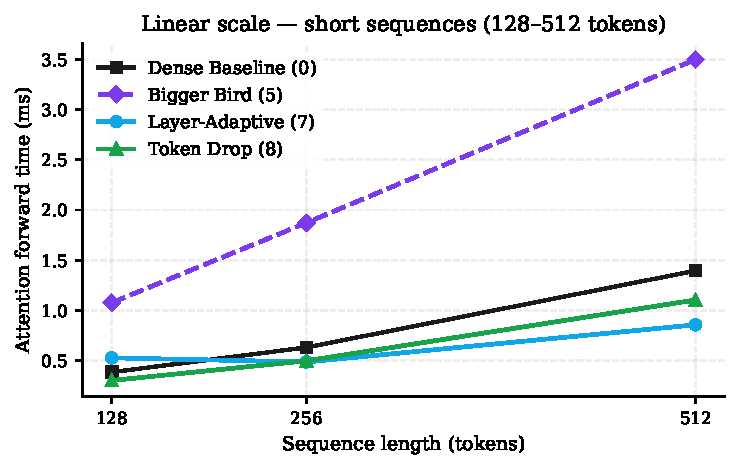
\includegraphics[width=\linewidth]{sel_linear_short}
    \caption{Short sequences (128--512 tokens).}
    \label{fig:linshort}
  \end{subfigure}
  \hfill
  \begin{subfigure}[b]{0.48\linewidth}
    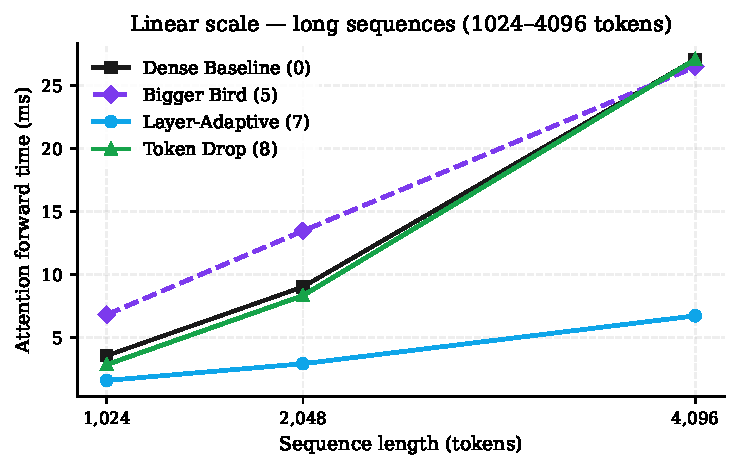
\includegraphics[width=\linewidth]{sel_linear_long}
    \caption{Long sequences (1024--4096 tokens).}
    \label{fig:linlong}
  \end{subfigure}
  \caption{Attention-kernel time on a linear scale for Dense Baseline (0),
  Bigger Bird Unified (5), Layer-Adaptive Sparsity (7), and Token Dropping (8).
  Dynamic Context (13) has no kernel benchmark and is omitted from these panels;
  it appears in Figure~\ref{fig:efficiency}. Kernel times for all other
  experiments appear in Table~\ref{tab:app-kernel}.}
  \label{fig:linear}
\end{figure}

Tables~\ref{tab:short} and~\ref{tab:long} present the same measurements on a
linear time axis. At 128 tokens, fixed routing and gather overhead can make
sparse methods slower than dense attention; most methods cross over between
256 and 512 tokens. At longer lengths the gap widens rapidly: from 1024 to
4096 tokens, dense attention grows by 7.7$\times$ while DeepSeek Top-k grows
by 3.7$\times$.

\begin{table}[ht]
  \centering
  \small
  \caption{Attention-forward time (ms), short sequences (128--512 tokens),
  linear scale.}
  \label{tab:short}
  \begin{tabular}{@{}lrrr@{}}
    \toprule
    Method & 128 & 256 & 512 \\
    \midrule
    Dense baseline (0)        & 0.386 & 0.632 & 1.396 \\
    DeepSeek Top-k (1)        & 0.463 & 0.487 & 0.858 \\
    Lightning Hybrid (2)      & 1.157 & 2.209 & 4.277 \\
    Dynamic Globals (3)       & 0.873 & 1.432 & 2.642 \\
    PBS Attn (4)              & 0.307 & 0.580 & 0.915 \\
    Bigger Bird Unified (5)   & 1.078 & 1.872 & 3.499 \\
    DeepSeek+PBS (6)          & 0.809 & 0.783 & 0.974 \\
    Layer-Adaptive (7)        & 0.528 & 0.487 & 0.857 \\
    Token Drop (8)            & 0.303 & 0.499 & 1.105 \\
    Attn Speculation (9)      & 0.745 & 1.294 & 2.433 \\
    GQA+Sparse (10)           & 0.493 & 0.503 & 0.883 \\
    \bottomrule
  \end{tabular}
\end{table}

\begin{table}[ht]
  \centering
  \small
  \caption{Attention-forward time (ms), long sequences (1024--4096 tokens),
  linear scale.}
  \label{tab:long}
  \begin{tabular}{@{}lrrr@{}}
    \toprule
    Method & 1024 & 2048 & 4096 \\
    \midrule
    Dense baseline (0)        & 3.537 & 9.007  & 27.092 \\
    DeepSeek Top-k (1)        & 1.567 & 2.889  & 5.834 \\
    Lightning Hybrid (2)      & 8.783 & 17.406 & 34.411 \\
    Dynamic Globals (3)       & 5.068 & 9.940  & 19.447 \\
    PBS Attn (4)              & 1.663 & 3.068  & 6.162 \\
    Bigger Bird Unified (5)   & 6.798 & 13.455 & 26.502 \\
    DeepSeek+PBS (6)          & 1.678 & 3.014  & 6.147 \\
    Layer-Adaptive (7)        & 1.567 & 2.897  & 6.707 \\
    Token Drop (8)            & 2.823 & 8.315  & 27.085 \\
    Attn Speculation (9)      & 4.722 & 9.451  & 18.575 \\
    GQA+Sparse (10)           & 1.595 & 2.961  & 6.925 \\
    \bottomrule
  \end{tabular}
\end{table}

Lightning Hybrid and Bigger Bird Unified remain slower than dense attention
at every tested length in the long-sequence table. Token Dropping is fast at
1024--2048 tokens but rejoins the dense kernel near 4096 tokens because its
first three layers remain dense. This kernel-only behavior does not represent
its complete end-to-end advantage, which appears once later-layer sequence
reduction affects training, latency, and memory
(Section~\ref{sec:efficiency}).

\subsection{Efficiency Metrics: F1, Latency, Memory, and Training Time}
\label{sec:efficiency}

\begin{figure}[ht]
  \centering
  \begin{subfigure}[b]{0.49\linewidth}
    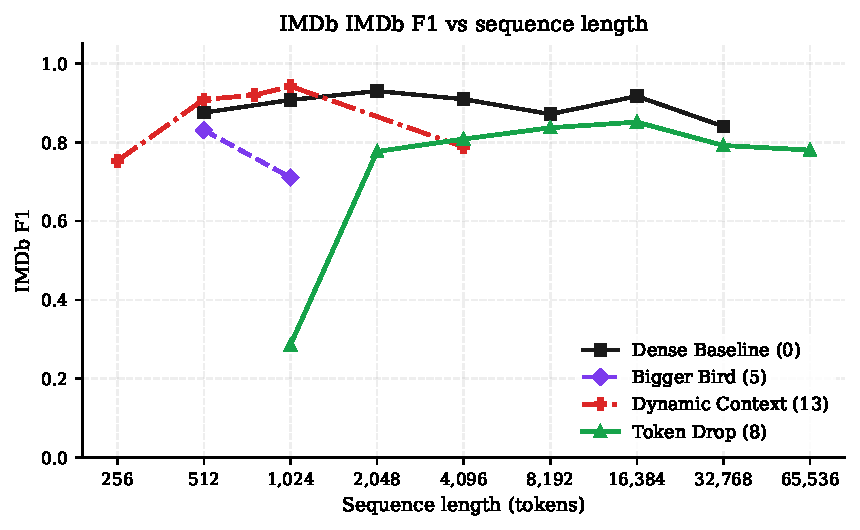
\includegraphics[width=\linewidth]{sel_f1}
    \caption{IMDb F1 vs sequence length.}
    \label{fig:f1seq}
  \end{subfigure}
  \hfill
  \begin{subfigure}[b]{0.49\linewidth}
    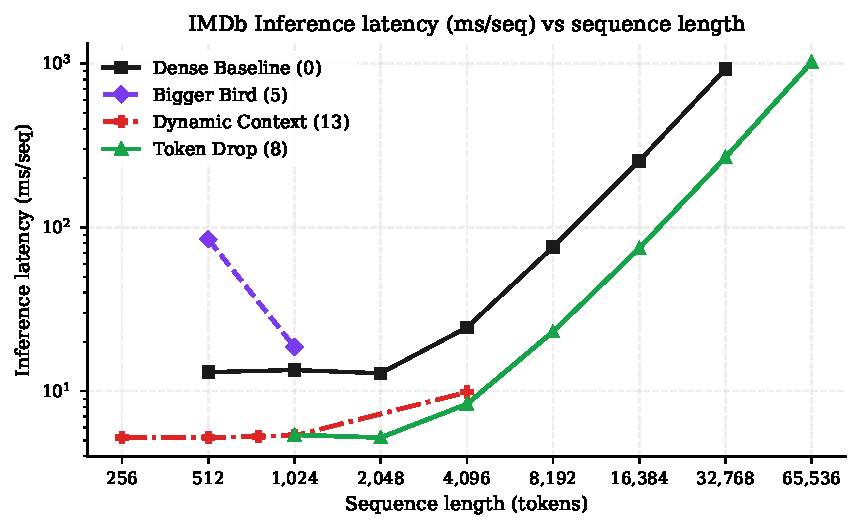
\includegraphics[width=\linewidth]{sel_latency}
    \caption{Inference latency vs sequence length.}
    \label{fig:latseq}
  \end{subfigure}

  \medskip
  \begin{subfigure}[b]{0.49\linewidth}
    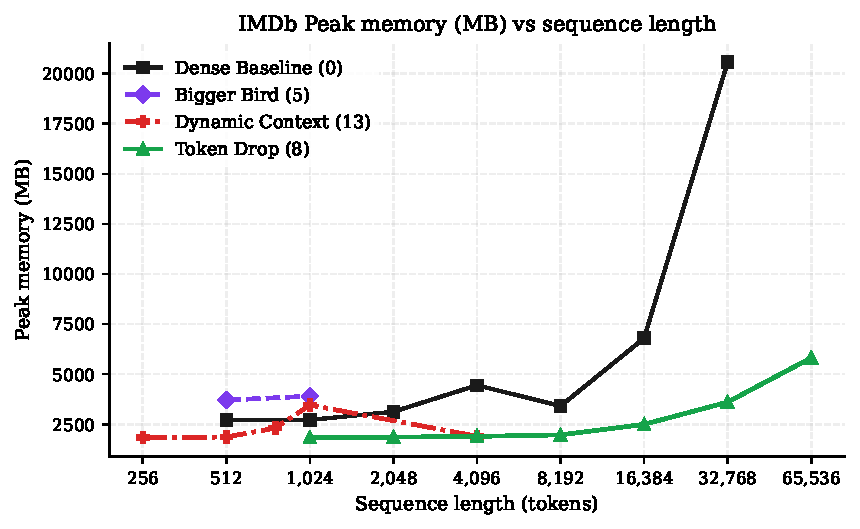
\includegraphics[width=\linewidth]{sel_memory}
    \caption{Peak device memory vs sequence length.}
    \label{fig:memseq}
  \end{subfigure}
  \hfill
  \begin{subfigure}[b]{0.49\linewidth}
    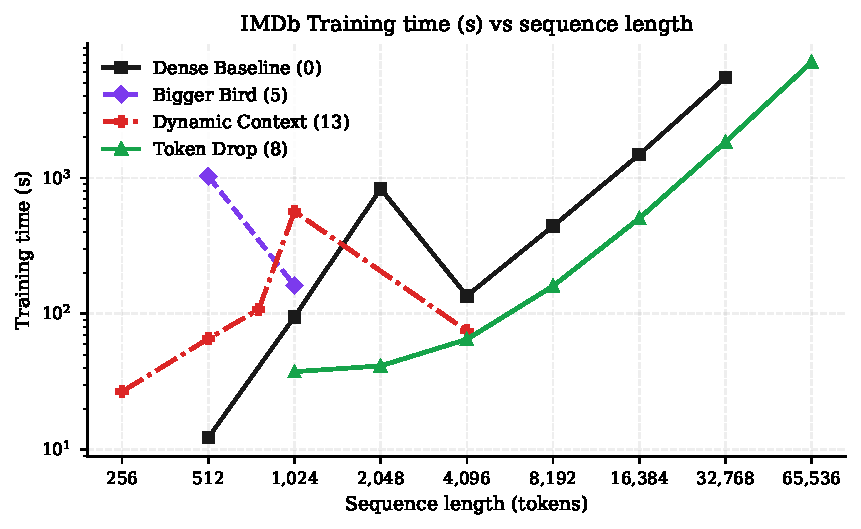
\includegraphics[width=\linewidth]{sel_traintime}
    \caption{Training time vs sequence length.}
    \label{fig:trainseq}
  \end{subfigure}

  \caption{IMDb task-level efficiency for the four highlighted experiments:
  Dense Baseline (0), Bigger Bird Unified (5), and the two top-performing
  alternatives by overall score: Dynamic Context (13) and Token Dropping (8).
  Overall score is the mean of six normalized axes --- F1, accuracy, inference
  speed, memory efficiency, training efficiency, and sparsity --- averaged
  across all recorded sequence lengths. Full results for all remaining
  experiments appear in Table~\ref{tab:app-imdb}.}
  \label{fig:efficiency}
\end{figure}

The panels compare task-level F1, latency, memory, and training time. The
detailed tables add DeepSeek Top-k because it has broad length coverage; all
other results appear in Table~\ref{tab:app-imdb}. An em-dash denotes a missing
metric, and OOM denotes an out-of-memory failure.

\begin{table}[ht]
  \centering
  \small
  \caption{Dense baseline (Experiment 0): IMDb efficiency by sequence length.}
  \label{tab:eff-baseline}
  \begin{tabular}{@{}rrrrr@{}}
    \toprule
    Seq.\ length & F1 & Train time (s) & Peak memory (MB) & Latency (ms) \\
    \midrule
    256    & 0.878 & 157.3   & ---      & ---   \\
    512    & 0.871 & 56.3    & 2707.4   & 13.68 \\
    768    & 0.931 & 216.7   & ---      & ---   \\
    1024   & 0.894 & 57.3    & 2725.4   & 13.18 \\
    2048   & 0.900 & 66.6    & 3061.0   & 13.21 \\
    4096   & 0.909 & 135.6   & 4446.4   & 24.47 \\
    8192   & 0.871 & 441.4   & 3408.8   & 75.72 \\
    16384  & 0.917 & 1484.9  & 6793.8   & 253.99 \\
    32768  & 0.840 & 5485.6  & 20{,}577.4 & 924.88 \\
    65536  & OOM   & OOM     & OOM      & OOM   \\
    \bottomrule
  \end{tabular}
\end{table}

\begin{table}[ht]
  \centering
  \small
  \caption{DeepSeek Top-k (Experiment 1): IMDb efficiency by sequence length.}
  \label{tab:eff-deepseek}
  \begin{tabular}{@{}rrrrr@{}}
    \toprule
    Seq.\ length & F1 & Train time (s) & Peak memory (MB) & Latency (ms) \\
    \midrule
    256    & 0.917 & 187.2  & ---      & ---   \\
    512    & 0.860 & 60.8   & 2701.4   & 16.07 \\
    768    & 0.926 & 609.8  & ---      & ---   \\
    1024   & 0.820 & 61.6   & 2726.6   & 15.00 \\
    2048   & 0.519 & 62.5   & 3077.6   & 15.08 \\
    4096   & 0.821 & 102.6  & 4385.7   & 20.40 \\
    8192   & 0.600 & 295.6  & 3390.2   & 53.94 \\
    16384  & 0.812 & 907.0  & 6791.6   & 168.21 \\
    32768  & 0.000 & 3170.7 & 20{,}577.1 & 581.10 \\
    65536  & OOM   & OOM    & OOM      & OOM   \\
    \bottomrule
  \end{tabular}
\end{table}

\begin{table}[ht]
  \centering
  \small
  \caption{Layer-Adaptive Sparsity (Experiment 7): IMDb efficiency by
  sequence length.}
  \label{tab:eff-layeradaptive}
  \begin{tabular}{@{}rrrrr@{}}
    \toprule
    Seq.\ length & F1 & Train time (s) & Peak memory (MB) & Latency (ms) \\
    \midrule
    512    & 0.800 & 118.1  & 2696.0   & 19.58 \\
    1024   & 0.891 & 84.5   & 2724.5   & 15.95 \\
    2048   & 0.830 & 81.3   & 2781.5   & 15.59 \\
    4096   & 0.864 & 124.6  & 2817.0   & 21.88 \\
    8192   & 0.826 & 298.1  & 3406.6   & 54.63 \\
    16384  & 0.842 & 911.5  & 6792.8   & 169.32 \\
    32768  & 0.778 & 3178.2 & 20{,}575.9 & 582.94 \\
    65536  & OOM   & OOM    & OOM      & OOM   \\
    \bottomrule
  \end{tabular}
\end{table}

\begin{table}[ht]
  \centering
  \small
  \caption{Token Dropping (Experiment 8): IMDb efficiency by sequence length.}
  \label{tab:eff-tokendrop}
  \begin{tabular}{@{}rrrrr@{}}
    \toprule
    Seq.\ length & F1 & Train time (s) & Peak memory (MB) & Latency (ms) \\
    \midrule
    1024   & 0.286 & 37.5   & 1833.6   & 5.41 \\
    2048   & 0.776 & 41.3   & 1857.3   & 5.21 \\
    4096   & 0.808 & 64.8   & 1894.2   & 8.33 \\
    8192   & 0.837 & 159.9  & 1968.2   & 23.09 \\
    16384  & 0.851 & 503.3  & 2494.4   & 74.48 \\
    32768  & 0.792 & 1837.5 & 3603.6   & 266.92 \\
    65536  & 0.780 & 7112.3 & 5815.3   & 1019.87 \\
    \bottomrule
  \end{tabular}
\end{table}

\FloatBarrier
\begin{table}[H]
  \centering
  \small
  \caption{Dynamic Context (Experiment 13): IMDb efficiency by sequence
  length.}
  \label{tab:eff-dynamiccontext}
  \begin{tabular}{@{}rrrrr@{}}
    \toprule
    Seq.\ length & F1 & Train time (s) & Peak memory (MB) & Latency (ms) \\
    \midrule
    256    & 0.000 & 26.9  & 1826.8 & 5.31 \\
    512    & 0.909 & 65.5  & 1862.3 & 5.20 \\
    768    & 0.919 & 107.4 & 2311.6 & 5.30 \\
    1024   & 0.942 & 566.4 & 3457.7 & 5.35 \\
    4096   & 0.788 & 74.9  & 1898.6 & 9.85 \\
    \bottomrule
  \end{tabular}
\end{table}

Several patterns emerge across Tables~\ref{tab:eff-baseline}--\ref{tab:eff-dynamiccontext}.
Inference latency separates the methods most clearly: Dynamic Context holds
latency in the 5.2--9.9~ms range across every tested length, roughly
2.5--26$\times$ lower than dense attention at the same length, because its
fixed post-drop token budget bounds the amount of computation regardless of
input length. Token Dropping shows the same qualitative pattern at longer
lengths, overtaking dense attention's memory profile once the sequence is long
enough that the post-drop token count is meaningfully smaller than the full
sequence (from roughly 2048 tokens onward). DeepSeek Top-k and Layer-Adaptive
Sparsity track dense attention's memory footprint closely at short-to-medium
lengths (within a few percent at 512--2048 tokens) because their savings are
concentrated in comparison count rather than in the number of activations
stored, and their latency advantage over dense attention only becomes large
at 8192 tokens and beyond (53.9--54.6~ms versus 75.7~ms).

Quality is comparatively more volatile than efficiency: three of the five
methods (DeepSeek Top-k, Layer-Adaptive, and, to a lesser extent, Token
Dropping) each have at least one sequence length where F1 drops sharply below
neighboring lengths (DeepSeek Top-k: 0.519 at 2048 tokens versus 0.820 at 1024
and 0.821 at 4096; Token Dropping: 0.286 at 1024 tokens versus 0.776 at 2048).
These dips do not follow a consistent direction with sequence length and are
most plausibly attributable to training-run variance (sample count, epoch
count, and random seed all differ across individual runs) rather than to a
property of the mechanism itself; they argue for the matched, multi-seed
re-run recommended in Section~\ref{sec:limitations}.

Table~\ref{tab:quality-1024} isolates the 1024-token comparison directly, and
Table~\ref{tab:tradeoffs} restates the same data as relative speedups and
memory reductions against the dense baseline at representative lengths.

\begin{table}[H]
  \centering
  \small
  \caption{IMDb quality at sequence length 1024.}
  \label{tab:quality-1024}
  \begin{tabular}{@{}lrrr@{}}
    \toprule
    Method & F1 & $\Delta$F1 vs.\ dense & Accuracy \\
    \midrule
    Dense baseline & 0.894 & 0.000 & 0.900 \\
    Dynamic Context & \textbf{0.942} & +0.048 & \textbf{0.941} \\
    Layer-Adaptive & 0.891 & $-0.003$ & 0.900 \\
    Attention Speculation & 0.841 & $-0.053$ & 0.860 \\
    DeepSeek Top-k & 0.820 & $-0.074$ & 0.820 \\
    Token Drop & 0.286 & $-0.608$ & 0.600 \\
    \bottomrule
  \end{tabular}
\end{table}

\begin{table}[H]
  \centering
  \small
  \caption{Representative quality--efficiency trade-offs relative to the dense
  baseline. Speedups above one are favorable; negative memory reduction denotes
  an increase.}
  \label{tab:tradeoffs}
  \begin{tabular}{@{}rrrcrr@{}}
    \toprule
    Length & Method & $\Delta$F1 & Inference speedup & Memory reduction & Train speedup \\
    \midrule
    1024  & Dynamic Context & +0.048 & 2.46$\times$ & $-26.9$\% & 0.10$\times$ \\
    4096  & Layer-Adaptive & $-0.045$ & 1.12$\times$ & 36.6\% & 1.09$\times$ \\
    8192  & Token Drop & $-0.034$ & 3.28$\times$ & 42.3\% & 2.76$\times$ \\
    16384 & Token Drop & $-0.066$ & 3.41$\times$ & 63.3\% & 2.95$\times$ \\
    32768 & Token Drop & $-0.048$ & 3.47$\times$ & 82.5\% & 2.99$\times$ \\
    \bottomrule
  \end{tabular}
\end{table}

Comparison count alone is not an adequate efficiency proxy. Dynamic Context at
1024 tokens reports about 1.85 billion softmax comparisons, versus 151 million
for dense attention, despite its much lower measured inference latency;
conversely, Layer-Adaptive at 4096 tokens reduces comparisons by 97.7\% but
improves end-to-end latency by only 12\%. Kernel overhead, the point at which
tokens are dropped, and the measurement boundary all need to be reported
alongside the comparison count, not in place of it.

\FloatBarrier
\subsection{BigBird-family developmental comparison}
\label{sec:bigbird-family-results}

Figure~\ref{fig:bigbirdfamily} summarizes an early BigBird-family comparison
at the two sequence lengths with matched family-level results. These runs
helped the team compare selection variants (globals, MMR, teleports) on a
shared encoder setup before moving to decoder long-context work. The
768-token panel tests whether the variants preserve baseline quality; the
8{,}000-token panel shows whether differences grow with context.

\begin{figure}[ht]
  \centering
  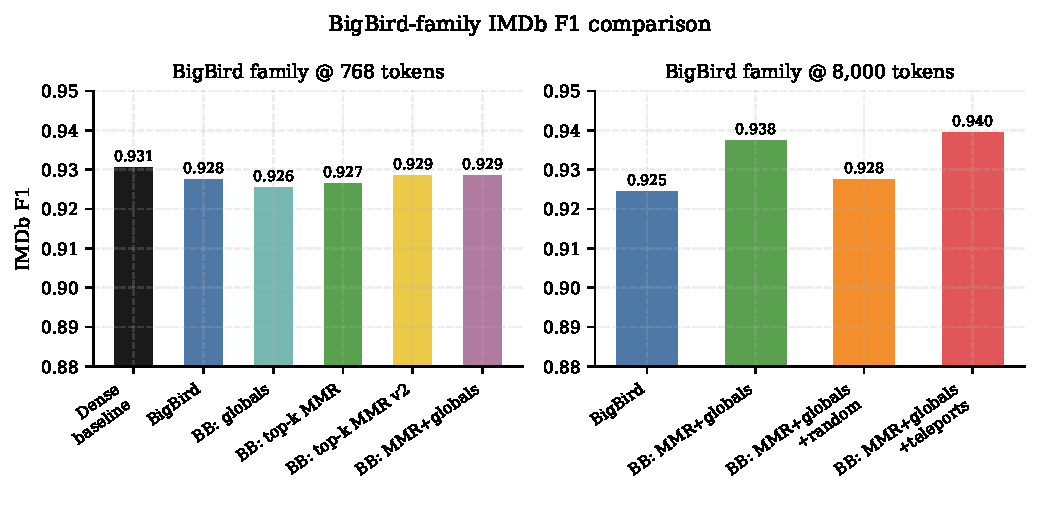
\includegraphics[width=\linewidth]{fig_bigbird_family}
  \caption{BigBird-family IMDb F1 at 768 tokens (left) and 8{,}000 tokens
  (right). All BigBird variants stay within 0.005 F1 of dense attention at
  768 tokens while training 12--14.7$\times$ slower; at 8{,}000 tokens
  the teleport-augmented variant reaches the family's best F1 (0.940) in
  4.9$\times$ less time than plain BigBird.}
  \label{fig:bigbirdfamily}
\end{figure}

At 768 tokens, all variants cluster within 0.005 F1 of the dense baseline, so
the figure shows little evidence of a meaningful quality separation at short
context. At 8{,}000 tokens, the teleport-augmented variant separates from
plain BigBird and the random-link variant, suggesting that targeted teleports
are more useful than additional random connections in this configuration.

Table~\ref{tab:bigbird-family} compares standard BigBird and four Bigger Bird
variants (Section~\ref{exp:bigbird-family}) against dense attention and the
unified design (Experiment~5) at 768 tokens. All BigBird-family variants land
within 0.005 F1 of dense attention, but every one of them trains
12--14.7$\times$ slower.

\begin{table}[ht]
  \centering
  \small
  \caption{BigBird-family IMDb results at sequence length 768.}
  \label{tab:bigbird-family}
  \begin{tabular}{@{}lrrr@{}}
    \toprule
    Method & F1 & Accuracy & Training time (s) \\
    \midrule
    Dense baseline & 0.931 & 0.931 & 216.7 \\
    BigBird & 0.928 & 0.931 & 2766.6 \\
    Bigger Bird: globals & 0.926 & 0.929 & 3055.8 \\
    Bigger Bird: top-k MMR & 0.927 & 0.930 & 2902.7 \\
    Bigger Bird: top-k MMR v2 & 0.929 & 0.932 & 2929.3 \\
    Bigger Bird: top-k MMR + globals & 0.929 & 0.932 & 3184.5 \\
    \bottomrule
  \end{tabular}
\end{table}

Table~\ref{tab:bigbird-family} also exposes the main short-context trade-off:
the methods retain nearly identical F1 and accuracy, but require
12--14.7$\times$ the dense baseline's training time. Thus, the 768-token
results support quality preservation, not a training-efficiency advantage.

At the longer 8{,}000-token IMDb configuration, the family separates further:
BigBird reaches F1~0.925 in 21{,}504~s of training, while Bigger Bird with
top-k~MMR + globals + teleports reaches the family's best F1 (0.940) in only
4348.7~s -- a 4.9$\times$ training-time reduction over plain BigBird at
comparable or better quality (Table~\ref{tab:bigbird-8000}).

\begin{table}[ht]
  \centering
  \small
  \caption{BigBird-family IMDb results at sequence length 8000.}
  \label{tab:bigbird-8000}
  \begin{tabular}{@{}lrrr@{}}
    \toprule
    Method & F1 & Accuracy & Training time (s) \\
    \midrule
    BigBird & 0.925 & 0.928 & 21{,}504.5 \\
    Bigger Bird: top-k MMR + globals & 0.938 & 0.940 & 7484.3 \\
    Bigger Bird: top-k MMR + globals + random & 0.928 & 0.930 & 5832.9 \\
    Bigger Bird: top-k MMR + globals + teleports & \textbf{0.940} & \textbf{0.941} & \textbf{4348.7} \\
    \bottomrule
  \end{tabular}
\end{table}

Table~\ref{tab:bigbird-8000} shows that teleports provide the strongest
combined result: F1 improves from 0.925 to 0.940 while training time falls by
about 80\% relative to plain BigBird. The comparison remains preliminary,
however, because these runs should be repeated under the matched protocol
described in Section~\ref{sec:limitations}.

\FloatBarrier
\section{Discussion}

The primary claim rests on the matched R1 evaluation: Bigger Bird v3 preserves
dense multiple-choice quality closely on long-context prompts while improving
mean prefill on the longer suites, with the speed crossover appearing beyond
the local-window regime. Decode speed is essentially unchanged without
eviction; the eviction arm matches first-token answers by construction and
should not be read as a long-generation quality result.

The developmental IMDb / kernel experiments explain how the project arrived
here. They were small-scale relative to Exp~20, but they made the scaling
behavior of routing, token dropping, and hybrid patterns visible early, and
they justified investing in content-based selection rather than fixed sparse
graphs alone. DeepSeek Top-k, Layer-Adaptive, and GQA Sparse showed strong
isolated kernel scaling; Token Dropping and Dynamic Context offered distinct
quality--efficiency profiles. Later R1 screens then showed that untrained
learned routers and undersized budgets fail synthetic retrieval, which is why
Bigger Bird v3 keeps sinks, a large window, routed distant keys, and an exact
tail. In short, the encoder work is the rationale and scaling scaffold; the
R1 suite is the current evidence.

\section{Limitations}
\label{sec:limitations}

R1 timings used short warmups, and the resolved upstream R1 weight revision
was not recorded in Modal metadata. Code.Debug and LongBench~v2 prompts beyond
130K were middle-truncated. The LongCodeQA 1M pilot covers 18/50 prompts under a
no-KV-cache protocol and must not be merged with the R1 128K-class table or
with Nemotron synthetic 1M runs. First-token A--D scores are not patch repair,
CoT generation quality, or long-decode quality after eviction. Published
methods such as DSA, LSA, and ZHA were not run under our matched protocol.

The developmental IMDb / kernel experiments use unequal training budgets,
incomplete metric fields, and single-run estimates, so they support design
rationale and qualitative scaling more than definitive encoder rankings.
``Bigger Bird'' historically referred to Experiment~5 (BART), Experiment~15
(BigBird-RoBERTa), Experiment~19 (Flash prototype), and the current v3 method;
readers should rely on the explicit version and experiment number.

\section{Conclusions and Recommendations}

Bigger Bird v3 is a context-aware sparse-prefill method for long-context
decoder inference. On the matched H100 R1 suite, it remains close to dense
A--D accuracy while improving prefill on longer prompts. Next steps are
completing the remaining 1M LongCodeQA prompts, longer-generation and
eviction quality tests, sparse-attention training, and matched comparisons
against recent inference-time sparse methods.


\clearpage
\addcontentsline{toc}{section}{References}
\bibliographystyle{IEEEtranN}
\bibliography{references}

\clearpage
\appendix
\section*{Appendix: Developmental Encoder Full Tables}
\addcontentsline{toc}{section}{Appendix: Developmental Encoder Full Tables}

This appendix reports the full IMDb / kernel tables from the early architecture
search (Section~\ref{sec:developmental}). These smaller-scale runs support
design rationale and scaling trends; they are not the primary R1 long-context
evidence. Experiments highlighted in the developmental section are: Dense
Baseline (0), Bigger Bird Unified (5), Dynamic Context (13), and Token
Dropping (8).

\subsection*{A.1\quad Attention-Kernel Forward Time (ms)}
OOM denotes an out-of-memory failure; `---' denotes not benchmarked at that length.

\begin{table}[ht]
  \centering
  \small
  \caption{Attention-kernel forward time (ms) for omitted experiments, 128--4096 tokens.}
  \label{tab:app-kernel}
  \begin{tabular}{@{}lrrrrrr@{}}
    \toprule
    Experiment & 128 & 256 & 512 & 1,024 & 2,048 & 4,096 \\
    \midrule
    GQA+Sparse & 0.493 & 0.503 & 0.883 & 1.595 & 2.961 & 6.925 \\
    DeepSeek Top-k & 0.463 & 0.487 & 0.858 & 1.567 & 2.889 & 5.834 \\
    Lightning Hybrid & 1.157 & 2.209 & 4.277 & 8.783 & 17.406 & 34.411 \\
    Dynamic Global Tokens & 0.873 & 1.432 & 2.642 & 5.068 & 9.940 & 19.447 \\
    PBS Attention & 0.307 & 0.580 & 0.915 & 1.663 & 3.068 & 6.162 \\
    DeepSeek+PBS Hybrid & 0.809 & 0.783 & 0.974 & 1.678 & 3.014 & 6.147 \\
    Attention Speculation & 0.745 & 1.294 & 2.433 & 4.722 & 9.451 & 18.575 \\
    \bottomrule
  \end{tabular}
\end{table}

\FloatBarrier

\subsection*{A.2\quad IMDb Task-Level Results (All Sequence Lengths)}
F1 = 0.000 with accuracy $\approx$ 0.53 indicates majority-class collapse.
OOM rows are included where recorded. `---' denotes metric not recorded.

\begingroup
\small
\setlength{\tabcolsep}{3pt}
\renewcommand{\addlinespace}[1][]{}
\newenvironment{appresultstable}{%
  \begin{center}
  \begin{tabular}{@{}>{\raggedright\arraybackslash}p{0.35\textwidth}lrrrrr@{}}
  \toprule
  Experiment & Seq & F1 & Acc & Train (s) & Mem. (MB) & Lat. (ms) \\
  \midrule
}{%
  \end{tabular}
  \end{center}
}
\captionsetup{hypcap=false}
\captionof{table}{IMDb task-level results for all experiments not in the main figures.}
\label{tab:app-imdb}
\begin{appresultstable}
  DeepSeek Top-k & 256 & 0.677 & 0.580 & 223.7 & --- & --- \\
   & 512 & 0.860 & 0.860 & 60.8 & 2701 & 16.07 \\
   & 1,024 & 0.846 & 0.840 & 100.5 & 2718 & 15.78 \\
   & 2,048 & 0.873 & 0.873 & 678.1 & 3124 & 15.30 \\
   & 4,096 & 0.837 & 0.840 & 131.5 & 2815 & 20.69 \\
   & 8,192 & 0.600 & 0.680 & 295.6 & 3390 & 53.94 \\
   & 16,384 & 0.812 & 0.820 & 907.0 & 6792 & 168.21 \\
   & 32,768 & 0.000 & 0.530 & 3170.7 & 20577 & 581.10 \\
   & 65,536 & \multicolumn{5}{l}{OOM} \\
  \addlinespace[4pt]
  Lightning Hybrid & 256 & 0.000 & 0.530 & 49.7 & 2806 & 47.37 \\
   & 512 & 0.775 & 0.770 & 10731.5 & 6034 & 73.68 \\
   & 1,024 & 0.750 & 0.600 & 2.3 & 2793 & 20.38 \\
   & 2,048 & 0.829 & 0.832 & 2603.4 & 7423 & 28.68 \\
   & 4,096 & 0.621 & 0.670 & 274.4 & 13956 & 52.25 \\
  \addlinespace[4pt]
\end{appresultstable}
\clearpage
\begin{appresultstable}
  Dynamic Global Tokens & 256 & 0.541 & 0.660 & 278.2 & --- & --- \\
   & 1,024 & 0.295 & 0.570 & 123.7 & 2716 & 18.54 \\
   & 2,048 & 0.840 & 0.842 & 2144.3 & 4999 & 21.33 \\
   & 4,096 & 0.000 & 0.530 & 281.8 & 3512 & 36.92 \\
  \addlinespace[4pt]
  PBS Attention & 256 & 0.550 & 0.640 & 317.2 & --- & --- \\
   & 512 & 0.000 & 0.560 & 13.1 & 2705 & 15.52 \\
   & 1,024 & 0.000 & 0.530 & 104.7 & 2716 & 15.37 \\
   & 2,048 & 0.656 & 0.488 & 698.5 & 3132 & 15.81 \\
   & 4,096 & 0.000 & 0.530 & 132.7 & 2815 & 21.12 \\
  \addlinespace[4pt]
  DeepSeek+PBS Hybrid & 512 & 0.000 & 0.530 & 128.0 & 2696 & 20.50 \\
   & 1,024 & \multicolumn{5}{l}{OOM} \\
   & 2,048 & \multicolumn{5}{l}{OOM} \\
   & 4,096 & \multicolumn{5}{l}{OOM} \\
  \addlinespace[4pt]
  Layer-Adaptive Sparsity & 512 & 0.848 & 0.850 & 99.2 & 2696 & 14.70 \\
   & 1,024 & 0.891 & 0.900 & 84.5 & 2725 & 15.95 \\
   & 2,048 & 0.901 & 0.901 & 687.5 & 3120 & 15.02 \\
   & 4,096 & 0.864 & 0.880 & 124.6 & 2817 & 21.88 \\
   & 8,192 & 0.826 & 0.840 & 298.1 & 3407 & 54.63 \\
   & 16,384 & 0.842 & 0.850 & 911.5 & 6793 & 169.32 \\
   & 32,768 & 0.778 & 0.800 & 3178.2 & 20576 & 582.94 \\
   & 65,536 & \multicolumn{5}{l}{OOM} \\
  \addlinespace[4pt]
  Attention Speculation & 1,024 & 0.841 & 0.860 & 132.5 & 4113 & 16.61 \\
   & 2,048 & 0.860 & 0.860 & 253.4 & 9395 & 21.00 \\
   & 4,096 & \multicolumn{5}{l}{OOM} \\
  \addlinespace[4pt]
  GQA+Sparse & 512 & 0.000 & 0.530 & 119.6 & 2696 & 19.63 \\
   & 1,024 & 0.763 & 0.770 & 107.2 & 2714 & 15.50 \\
   & 2,048 & 0.796 & 0.800 & 121.5 & 2779 & 21.95 \\
   & 4,096 & 0.750 & 0.800 & 123.2 & 2817 & 22.30 \\
  \addlinespace[4pt]
  Native Sparse Attn (NSA) & \multicolumn{6}{l}{No task-level run recorded} \\
  S2-HHST & \multicolumn{6}{l}{No task-level run recorded} \\
  Token Drop + DeepSeek & 4,096 & 0.641 & 0.485 & 67.9 & 17100 & 17.61 \\
   & 8,192 & 0.041 & 0.530 & 246.6 & 33011 & 62.81 \\
   & 16,384 & \multicolumn{5}{l}{OOM} \\
   & 32,768 & \multicolumn{5}{l}{OOM} \\
   & 65,536 & \multicolumn{5}{l}{OOM} \\
  \addlinespace[4pt]
  Bigger Bird (BigBird-RoBERTa) & \multicolumn{6}{l}{No task-level run recorded} \\
\end{appresultstable}
\clearpage
\begin{appresultstable}
  lra_text_exp_7_layer_adaptive & 512 & 0.649 & 0.480 & 60.7 & 950 & 15.02 \\
   & 1,024 & 0.649 & 0.480 & 123.1 & 1527 & 24.06 \\
   & 2,048 & 0.649 & 0.480 & 263.5 & 2724 & 51.59 \\
   & 4,096 & 0.649 & 0.480 & 26.2 & 3868 & 8.54 \\
   & 8,192 & 0.000 & 0.438 & 37.6 & 2902 & 259.83 \\
   & 16,384 & 0.000 & 0.520 & 199.5 & 2586 & 20.67 \\
   & 32,768 & 0.000 & 0.520 & 542.9 & 6836 & 45.89 \\
  \addlinespace[4pt]
  lra_text_exp_11_nsa & 1,024 & 0.000 & 0.438 & 797.4 & 8941 & 79.09 \\
  \addlinespace[4pt]
  lra_listops_exp_11_nsa & 512 & 0.060 & 0.135 & 9541.5 & 15508 & 40.18 \\
  \addlinespace[4pt]
  ruler_niah_exp_2_lightning_hybrid & 4,096 & 0.016 & 0.085 & 900.0 & 30138 & 43.10 \\
   & 8,192 & 0.021 & 0.120 & 1815.4 & 30202 & 93.09 \\
   & 16,384 & 0.017 & 0.090 & 4140.7 & 7365 & 196.94 \\
  \addlinespace[4pt]
  lra_listops_exp_2_lightning_hybrid & 512 & 0.024 & 0.135 & 1249.1 & 7475 & 24.37 \\
   & 1,024 & 0.023 & 0.130 & 4093.7 & 14799 & 48.17 \\
  \addlinespace[4pt]
  ruler_niah_exp_1_deepseek_topk & 4,096 & 0.016 & 0.085 & 52.9 & 3530 & 8.32 \\
   & 8,192 & 0.021 & 0.120 & 113.2 & 3601 & 9.78 \\
   & 16,384 & 0.017 & 0.090 & 344.9 & 1562 & 20.02 \\
   & 32,768 & 0.019 & 0.105 & 770.5 & 2740 & 44.49 \\
  \addlinespace[4pt]
  lra_text_exp_3_dynamic_globals & 1,024 & 0.000 & 0.438 & 10.4 & 2170 & 35.91 \\
   & 2,048 & 0.000 & 0.438 & 16.9 & 4032 & 76.44 \\
   & 4,096 & 0.000 & 0.438 & 363.6 & 7739 & 162.47 \\
   & 8,192 & 0.000 & 0.438 & 922.9 & 15164 & 363.20 \\
  \addlinespace[4pt]
  lra_text_exp_14_token_drop_deepseek & 4,096 & 0.641 & 0.485 & 67.9 & 17100 & 17.61 \\
   & 8,192 & 0.041 & 0.530 & 246.6 & 33011 & 62.81 \\
  \addlinespace[4pt]
  ruler_niah_exp_7_layer_adaptive & 4,096 & 0.016 & 0.085 & 54.6 & 3676 & 9.06 \\
   & 8,192 & 0.021 & 0.120 & 118.7 & 3746 & 10.35 \\
   & 16,384 & 0.017 & 0.090 & 348.7 & 1562 & 20.60 \\
  \addlinespace[4pt]
  biggerbird_topk_mmr & 768 & 0.927 & 0.930 & 2902.7 & --- & --- \\
  \addlinespace[4pt]
  lra_text_exp_12_s2_hhst & 1,024 & 0.000 & 0.438 & 318.9 & 6532 & 50.45 \\
  \addlinespace[4pt]
  lra_listops_exp_3_dynamic_globals & 512 & 0.034 & 0.140 & 166.3 & 4076 & 20.28 \\
   & 1,024 & 0.023 & 0.130 & 3705.6 & 7760 & 35.03 \\
  \addlinespace[4pt]
\end{appresultstable}
\clearpage
\begin{appresultstable}
  lra_listops_exp_5_bigger_bird & 512 & 0.042 & 0.135 & 1090.2 & 5548 & 25.30 \\
   & 1,024 & 0.030 & 0.135 & 8795.5 & 14803 & 45.27 \\
  \addlinespace[4pt]
  lra_listops_exp_10_gqa_sparse & 512 & 0.033 & 0.140 & 59.9 & 950 & 18.25 \\
  \addlinespace[4pt]
  biggerbird_topkmmr+globals_ver1 & 768 & 0.929 & 0.932 & 3184.5 & --- & --- \\
  \addlinespace[4pt]
  lra_listops_exp_12_s2_hhst & 512 & 0.068 & 0.150 & 5728.8 & 9454 & 24.35 \\
  \addlinespace[4pt]
  ruler_niah_exp_6_deepseek_pbs & 4,096 & 0.016 & 0.085 & 53.6 & 3530 & 10.43 \\
   & 8,192 & 0.021 & 0.120 & 115.6 & 3601 & 11.70 \\
   & 16,384 & 0.017 & 0.090 & 357.2 & 1562 & 20.58 \\
  \addlinespace[4pt]
  lra_listops_exp_7_layer_adaptive & 256 & 0.023 & 0.133 & 11.2 & 841 & 12.20 \\
   & 512 & 0.052 & 0.140 & 60.6 & 949 & 17.00 \\
   & 1,024 & 0.023 & 0.130 & 122.7 & 1526 & 24.34 \\
   & 2,048 & 0.019 & 0.105 & 263.3 & 2722 & 51.68 \\
  \addlinespace[4pt]
  lra_text_exp_0_baseline & 256 & 0.646 & 0.477 & 44.5 & 684 & 28.36 \\
   & 512 & 0.649 & 0.480 & 71.0 & 946 & 14.24 \\
   & 1,024 & 0.649 & 0.480 & 170.2 & 1561 & 26.54 \\
   & 2,048 & 0.667 & 0.500 & 20.7 & 2955 & 67.15 \\
   & 4,096 & 0.000 & 0.438 & 33.1 & 1840 & 188.13 \\
   & 8,192 & 0.000 & 0.438 & 110.5 & 4293 & 582.79 \\
  \addlinespace[4pt]
  ruler_niah_exp_13_dynamic_context & 4,096 & 1.000 & 1.000 & 83.3 & 2646 & 7.70 \\
   & 8,192 & 0.021 & 0.120 & 185.9 & 2115 & 13.93 \\
   & 16,384 & 0.017 & 0.090 & 457.9 & 906 & 23.84 \\
   & 32,768 & 0.019 & 0.105 & 829.0 & 1283 & 43.44 \\
   & 65,536 & 0.021 & 0.120 & 1612.0 & 2005 & 82.77 \\
  \addlinespace[4pt]
  lra_text_exp_5_bigger_bird & 1,024 & 0.000 & 0.438 & 71.6 & 3930 & 45.84 \\
   & 2,048 & 0.000 & 0.438 & 701.2 & 11646 & 128.71 \\
  \addlinespace[4pt]
  lra_text_exp_2_lightning_hybrid & 1,024 & 0.000 & 0.438 & 12.2 & 3934 & 50.24 \\
   & 2,048 & 0.000 & 0.438 & 148.2 & 7546 & 122.45 \\
   & 4,096 & 0.649 & 0.480 & 356.4 & 30144 & 44.26 \\
   & 8,192 & 0.000 & 0.520 & 733.2 & 30210 & 93.02 \\
   & 32,768 & 0.000 & 0.520 & 3523.6 & 15374 & 401.49 \\
  \addlinespace[4pt]
  biggerbird_topkMMR_globals_teleports_8000 & 8,000 & 0.940 & 0.941 & 4348.7 & --- & --- \\
  \addlinespace[4pt]
  ruler_niah_exp_0_baseline & 512 & 0.027 & 0.156 & 525.0 & 0 & 247.83 \\
  \addlinespace[4pt]
  biggerbird_topk_mmr_ver2_(kaggle) & 768 & 0.929 & 0.932 & 2929.3 & --- & --- \\
  \addlinespace[4pt]
\end{appresultstable}
\clearpage
\begin{appresultstable}
  lra_text_exp_10_gqa_sparse & 1,024 & 0.000 & 0.438 & 4.2 & 584 & 23.22 \\
   & 2,048 & 0.000 & 0.438 & 7.3 & 884 & 49.24 \\
   & 4,096 & 0.000 & 0.438 & 15.1 & 1505 & 109.26 \\
   & 8,192 & 0.000 & 0.438 & 37.2 & 2853 & 257.82 \\
  \addlinespace[4pt]
  lra_text_exp_4_pbs_attn & 1,024 & 0.000 & 0.438 & 4.5 & 598 & 26.95 \\
   & 2,048 & 0.000 & 0.438 & 7.5 & 910 & 52.18 \\
   & 4,096 & 0.000 & 0.438 & 15.3 & 1554 & 111.76 \\
   & 8,192 & 0.000 & 0.438 & 37.8 & 2951 & 262.26 \\
  \addlinespace[4pt]
  lra_text_exp_9_attn_specul & 1,024 & 0.000 & 0.438 & 86.6 & 4294 & 35.00 \\
   & 2,048 & 0.000 & 0.438 & 641.3 & 12533 & 73.89 \\
  \addlinespace[4pt]
  lra_text_exp_8_token_drop & 512 & 0.649 & 0.480 & 47.5 & 890 & 10.50 \\
   & 1,024 & 0.649 & 0.480 & 109.8 & 1874 & 22.43 \\
   & 2,048 & 0.639 & 0.470 & 767.6 & 5221 & 62.11 \\
   & 4,096 & 0.649 & 0.480 & 98.2 & 20576 & 25.80 \\
   & 8,192 & 0.000 & 0.438 & 587.9 & 16040 & 2258.95 \\
  \addlinespace[4pt]
  ruler_niah_exp_14_token_drop_deepseek & 4,096 & 0.118 & 0.200 & 163.4 & 17100 & 17.62 \\
   & 8,192 & 0.021 & 0.120 & 588.4 & 33011 & 62.82 \\
  \addlinespace[4pt]
  lra_listops_exp_1_deepseek_topk & 256 & 0.016 & 0.086 & 11.3 & 841 & 11.91 \\
   & 512 & 0.024 & 0.135 & 60.6 & 950 & 21.29 \\
   & 1,024 & 0.033 & 0.105 & 121.3 & 1516 & 22.90 \\
   & 2,048 & 0.019 & 0.105 & 260.3 & 2669 & 51.06 \\
  \addlinespace[4pt]
  lra_text_exp_1_deepseek_topk & 256 & 0.000 & 0.523 & 11.1 & 842 & 14.95 \\
   & 512 & 0.649 & 0.480 & 61.1 & 951 & 15.14 \\
   & 1,024 & 0.649 & 0.480 & 122.8 & 1518 & 23.34 \\
   & 2,048 & 0.649 & 0.480 & 260.8 & 2671 & 51.07 \\
   & 4,096 & 0.649 & 0.480 & 25.5 & 3722 & 8.49 \\
   & 8,192 & 0.000 & 0.520 & 58.7 & 3985 & 9.75 \\
   & 16,384 & 0.000 & 0.520 & 194.5 & 2586 & 20.00 \\
   & 32,768 & 0.000 & 0.520 & 535.0 & 6836 & 44.47 \\
  \addlinespace[4pt]
  ruler_mq_niah_exp_13_dynamic_context & 4,096 & 1.000 & 1.000 & 84.6 & 2646 & 7.65 \\
   & 8,192 & 0.026 & 0.150 & 169.6 & 3769 & 13.93 \\
   & 16,384 & 0.017 & 0.090 & 300.5 & 6126 & 23.83 \\
   & 32,768 & 0.028 & 0.085 & 560.8 & 10747 & 43.51 \\
   & 65,536 & 0.017 & 0.095 & 1081.7 & 19987 & 82.70 \\
  \addlinespace[4pt]
  lra_listops_exp_4_pbs_attn & 512 & 0.025 & 0.090 & 61.3 & 980 & 16.99 \\
   & 1,024 & 0.023 & 0.130 & 121.6 & 1571 & 23.22 \\
  \addlinespace[4pt]
\end{appresultstable}
\clearpage
\begin{appresultstable}
  biggerbird_globals_ver1_(kaggle) & 768 & 0.926 & 0.929 & 3055.8 & --- & --- \\
  \addlinespace[4pt]
  ruler_niah_exp_8_token_drop & 4,096 & 0.016 & 0.085 & 236.0 & 20576 & 25.84 \\
  \addlinespace[4pt]
  biggerbird_topkMMR_globals_8000 & 8,000 & 0.938 & 0.940 & 7484.3 & --- & --- \\
  \addlinespace[4pt]
  lra_text_exp_13_dynamic_context & 4,096 & 0.641 & 0.480 & 33.7 & 2646 & 7.64 \\
   & 8,192 & 0.040 & 0.525 & 73.7 & 2115 & 13.91 \\
   & 16,384 & 0.078 & 0.530 & 180.0 & 906 & 23.86 \\
   & 32,768 & 0.020 & 0.520 & 325.6 & 1283 & 43.49 \\
   & 65,536 & 0.161 & 0.530 & 631.7 & 2005 & 82.76 \\
  \addlinespace[4pt]
  lra_listops_exp_6_deepseek_pbs & 512 & 0.025 & 0.090 & 60.5 & 950 & 17.24 \\
   & 1,024 & 0.052 & 0.165 & 119.6 & 1516 & 24.19 \\
  \addlinespace[4pt]
  lra_listops_exp_9_attn_specul & 512 & 0.016 & 0.085 & 1949.2 & 6188 & 19.69 \\
  \addlinespace[4pt]
  ruler_mq_niah_exp_8_token_drop & 4,096 & 0.021 & 0.120 & 236.9 & 20576 & 25.86 \\
  \addlinespace[4pt]
  lra_listops_exp_0_baseline & 256 & 0.023 & 0.133 & 44.5 & 683 & 28.91 \\
   & 512 & 0.018 & 0.095 & 70.1 & 944 & 14.08 \\
   & 1,024 & 0.025 & 0.140 & 168.6 & 1559 & 26.17 \\
   & 2,048 & 0.019 & 0.105 & 465.9 & 2953 & 68.99 \\
  \addlinespace[4pt]
  biggerbird_topkMMR_globals_randoms_8000 & 8,000 & 0.928 & 0.930 & 5832.9 & --- & --- \\
  \addlinespace[4pt]
  lra_listops_exp_8_token_drop & 512 & 0.044 & 0.115 & 46.5 & 888 & 10.30 \\
   & 1,024 & 0.046 & 0.140 & 109.5 & 1872 & 22.40 \\
   & 2,048 & 0.037 & 0.115 & 724.6 & 5219 & 62.24 \\
  \addlinespace[4pt]
  bigbird & 768 & 0.928 & 0.931 & 2766.6 & --- & --- \\
  \addlinespace[4pt]
  ruler_mq_niah_exp_14_token_drop_deepseek & 4,096 & 0.319 & 0.445 & 163.1 & 17100 & 17.63 \\
  \addlinespace[4pt]
  lra_text_exp_6_deepseek_pbs & 1,024 & 0.000 & 0.438 & 4.9 & 584 & 24.75 \\
   & 2,048 & 0.000 & 0.438 & 7.6 & 884 & 51.94 \\
   & 4,096 & 0.649 & 0.480 & 25.8 & 3722 & 10.20 \\
   & 8,192 & 0.000 & 0.520 & 59.9 & 3985 & 10.91 \\
   & 16,384 & 0.000 & 0.520 & 201.7 & 2586 & 20.33 \\
   & 32,768 & 0.000 & 0.520 & 537.2 & 6836 & 45.15 \\
  \addlinespace[4pt]
  bigbird_8000 & 8,000 & 0.925 & 0.928 & 21504.5 & --- & --- \\
  \addlinespace[4pt]
\end{appresultstable}
\endgroup


\end{document}